\section{Trabalhos Relacionados}
\label{subsection:trabalhoscorrelatos}
 Segundo \citeonline{tahawalid2009}, existem duas maneiras diferentes pelas quais um domínio pode ser definido. A primeira é quando o domínio está bem definido matematicamente, a segunda quando o domínio é definido por atividades puramente humanas. As DSLs de domínio humano, definem uma linguagem especial ou jargões para comunicar ideias relacionadas ao seu domínio.  
 
 Assim como a DSL Cotas, os trabalhos relacionados encontrados mostraram formas de modelar e abstrair conceitos e jargões envolvendo questões legais, contratuais e regras sobre domínios financeiros. Os domínios dessas DSLs foram definidos com objetivo de apoiar na compreensão de atividades humanas e não de tratar de problemas computacionais ou matemáticos.
 
 Para tanto, as DSLs descritas nas próximas Subseções foram encontradas por meio da busca pelas palavras-chave (domain specific languages, DSL, law e legal)  nos repositórios, \textit{Researchgate}, \textit{Google Scholar} e \textit{IEEEXplore}.
 
 
\subsection{LegalLanguage}
\label{legallanguage}

A DSL \texttt{LegalLanguage} é resultado da análise de ontologias que tratam de estrutura de documentos legais, sua construção busca estabelecer modelos conceituais com propósito de melhoria de comunicação e aprendizado sobre definições encontradas em textos normativos.

Apesar de tratar de domínio de questões legais, sua modelagem difere do presente trabalho pois a sua construção foi baseada em ontologias já existentes, com propósito de auxiliar em definições de documentos legais de maneira geral, enquanto a DSL Cotas foi modelada a partir do histórico de controle de versão entre as diferentes versões da legislação e trata especificamente da lei de cotas. 

\begin{figure}[ht!]
\centering

\caption{\textmd{Modelo da DSL LegalLanguage}}
\label{fig:legallanguagemodel}
\fcolorbox{gray}{white}{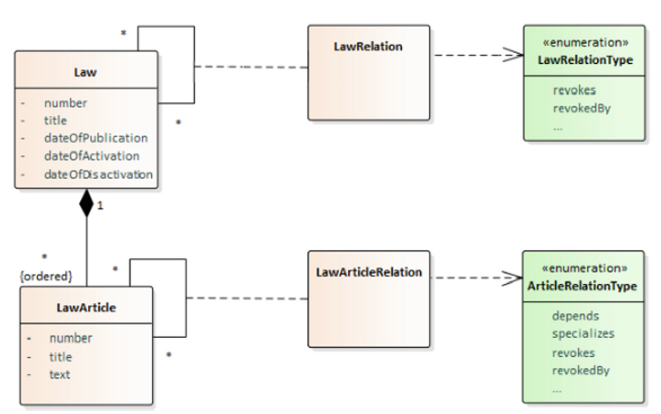
\includegraphics[width=0.90\textwidth]{chapters/trabalhoscorrelatos/imagens/legallanguagemodel.png}}

\par\medskip\textbf{Fonte:} \cite{legallanguage}. \par\medskip

\end{figure}



Segundo \citeonline{legallanguage}, o modelo da \texttt{LegalLanguage} é composto de \textit{Laws}, que podem ser classificadas como: Leis internacionais, regulamentos públicos, regulamentos privados, constituições e leis ordinárias. As leis são compostas por uma série de artigos ordenados sequencialmente, os quais são organizados em divisões. É possível criar relacionamentos hierárquicos entre artigos de diferentes elementos de lei, bem como indicar revogações quando novas leis surgem (Figura \ref{fig:legallanguagemodel}). 

\newpage
Ainda para esses autores: ''O desenvolvimento dessa linguagem tem como objetivo apoiar parlamentares que executam atividades inseridas em processos legislativos de redação de leis''  \cite[p. 45, tradução nossa]{legallanguage}. Portanto, os autores a criaram utilizando a ferramenta \texttt{Xtext}, um exemplo de definição e uso do elemento \texttt{Law} pode ser observado nas Figuras \ref{fig:xtextlegal} e \ref{fig:legallanguageexample}.

\begin{figure}[ht!]
\centering

\caption{\textmd{Definição do elemento Law na LegalLanguage}}
\label{fig:xtextlegal}
\fcolorbox{gray}{white}{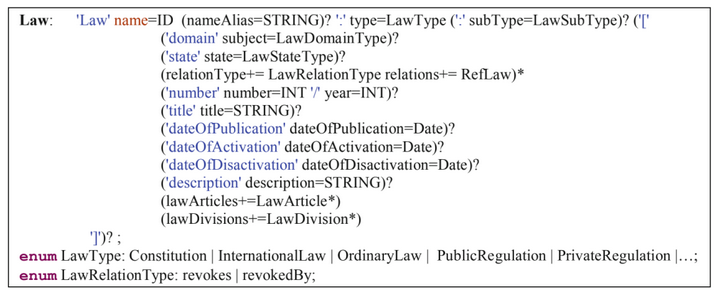
\includegraphics[width=\textwidth]{chapters/trabalhoscorrelatos/imagens/xtextlegal.png}}

\par\medskip\textbf{Fonte:} \citeonline{legallanguage}. \par\medskip

\end{figure}




\begin{figure}[ht!]
\centering

\caption{\textmd{Exemplo ilustrativo da LegalLanguage}}
\label{fig:legallanguageexample}
\fcolorbox{gray}{white}{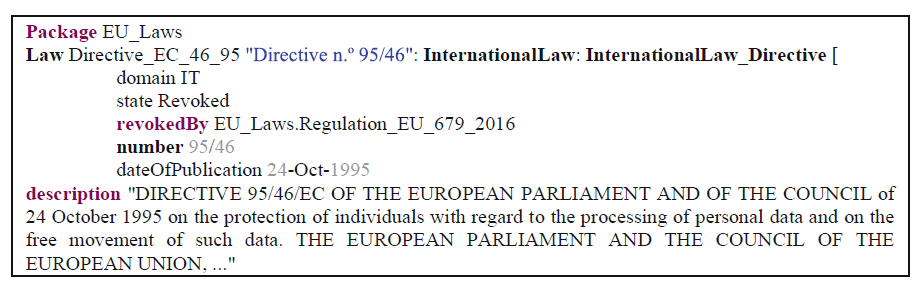
\includegraphics[width=\textwidth]{chapters/trabalhoscorrelatos/imagens/legallanguageexample.png}}

\par\medskip\textbf{Fonte:} \citeonline{legallanguage}. \par\medskip

\end{figure}





\newpage
\subsection{Ergo uma DSL para Contratos Legais Inteligentes}
\label{ergo}

Ergo é uma linguagem específica de domínio que faz parte do projeto Accord, o qual define a base jurídica e técnica para contratos legais inteligentes, com objetivo de atender aos problemas relacionados à falta de padronização em contratos legais. 

Segundo \citeonline{accordproject}, a linguagem tem o foco de ajudar desenvolvedores da área de tecnologia jurídica na escrita de contratos legais que possam ser computados. Um contrato legal inteligente é um contrato legível por seres humanos e por máquinas, por exemplo, uma cláusula de cobrança de pagamento pode estar presente em um contrato, de modo que se possa utilizar o texto descrito em linguagem natural, para extração dos dados de cobrança e posterior aplicação de cálculos de multas e geração de eventos de notificações. 

De forma similar a DSL Cotas, sua modelagem garante que as definições dos usuários sejam escritas com expressividade limitada, por outro lado, enquanto a DSL Cotas utiliza a definição das regras de distribuição de cotas em formato de tabelas, a Ergo DSL utiliza um formato textual controlado, similar ao de estrutura de classes para contratos e métodos para suas cláusulas.

É uma linguagem fortemente tipada e independente de plataforma, seu código pode ser compilado nas plataformas \texttt{JavaScript} e \texttt{Java}. Ela provê uma linguagem de expressões, pela qual é possível descrever funções e cláusulas de modo que possa ser definida a lógica de contratos inteligentes.

\newpage
Um exemplo de linguagem natural pode ser observado na Figura \ref{fig:ergotexto}, no qual os dados sobre a cláusula de cobrança são mapeados para posteriormente serem modelados e terem a lógica de cobrança seja definida (Figura \ref{fig:ergologica}). 

\begin{figure}[ht!]
\centering

\caption{\textmd{Exemplo ilustrativo da Ergo DSL}}
\label{fig:ergotexto}
\fcolorbox{gray}{white}{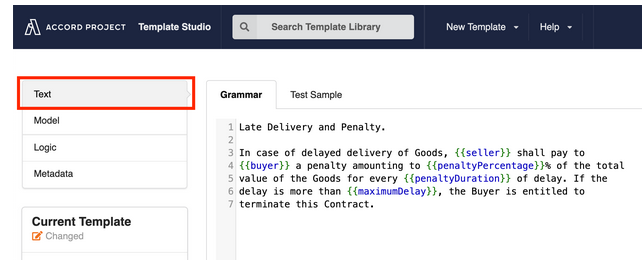
\includegraphics[width=\textwidth]{chapters/trabalhoscorrelatos/imagens/ergotexto.PNG}}

\par\medskip\textbf{Fonte:} \cite{accordproject}. \par\medskip

\end{figure}



\begin{figure}[ht!]
\centering

\caption{\textmd{Definição da lógica de contratos}}
\label{fig:ergologica}
\fcolorbox{gray}{white}{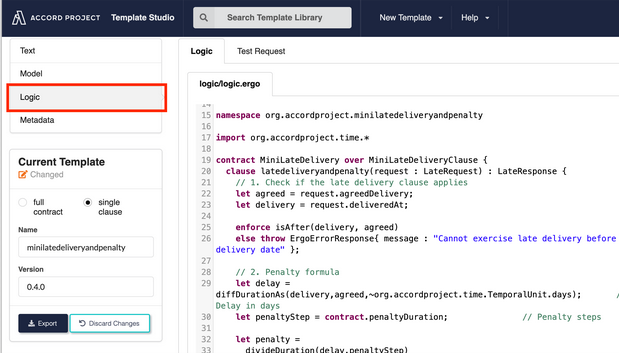
\includegraphics[width=\textwidth]{chapters/trabalhoscorrelatos/imagens/ergologica.PNG}}

\par\medskip\textbf{Fonte:} \citeonline{accordproject}. \par\medskip

\end{figure}




\clearpage

\subsection{DSL Capgemini Pension}
\label{capgeminipension}

Segundo \citeonline{gregfuller2013}, foi criada com o objetivo de atender ao domínio de planos de previdência e fornecimento de planos de seguros de pensão, no qual cada plano pode conter centenas de regras específicas, tratadas conforme o histórico de até 40 anos de dados funcionais para milhares de segurados. 

 Para \citeonline{kolkhenk2008}, essa linguagem advém da demanda de inovação em produtos da área e é baseada em interesses governamentais, no sentido de que há a necessidade de adequação às novas leis de pensão, dar transparência sobre as regras e fornecer garantia de qualidade. Portanto, essa DSL se relaciona ao presente trabalho no que diz respeito à necessidade de adequação, inovação e evolução para questões de interesses governamentais e para atendimento de novas legislações.

Criada com a ferramenta \texttt{Intentional Software} para construção de DSLs projecionais, ela permite que as definições das regras dos planos sejam realizadas em formato gráfico no estilo de tabelas de Excel (Figura \ref{fig:dslcapgeminitables}) e permite fazer testes unitários para validar as regras em tempo real (Figura \ref{fig:dslcapgeminiunittests}). 

\begin{figure}[ht!]
\centering

\caption{\textmd{Editor projecional das regras de pensão}}
\label{fig:dslcapgeminitables}
\fcolorbox{gray}{white}{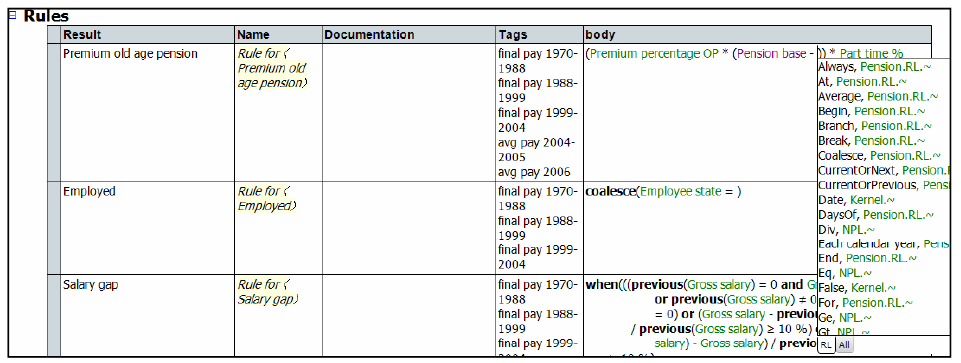
\includegraphics[width=\textwidth]{chapters/trabalhoscorrelatos/imagens/dslcapgeminitables.PNG}}

\par\medskip\textbf{Fonte:} \citeonline{kolkhenk2008}. \par\medskip

\end{figure}



\begin{figure}[ht!]
\centering

\caption{\textmd{Testes unitários das regras}}
\label{fig:dslcapgeminiunittests}
\fcolorbox{gray}{white}{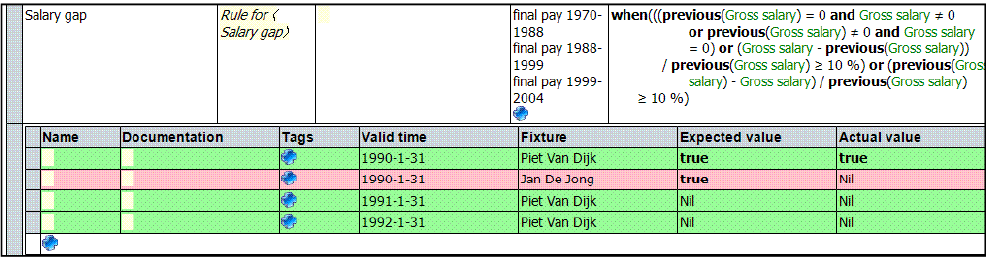
\includegraphics[width=\textwidth]{chapters/trabalhoscorrelatos/imagens/dslcapgeminiunittests.png}}

\par\medskip\textbf{Fonte:} \citeonline{kolkhenk2008}. \par\medskip

\end{figure}



O ambiente da linguagem substitui uma série de planilhas, documentos de texto e outras fontes de controle utilizadas por múltiplos especialistas de domínio no contexto de gerenciamento dos planos de pensão. Dessa forma, a \textit{Pension Workbench} traz um ambiente colaborativo controlado, com sistema integrado de controle de versão, sendo passível criar testes unitários e gerar a \textit{engine} responsável pelos cálculos para a administração dos planos e fundos de pensão \cite{gregfuller2013}.

Portanto, esses trabalhos relacionados assemelham-se à presente pesquisa no sentido de abordarem DSLs como meio de abstração de conhecimento de negócio. Eles visam a melhoria de processos que necessitem de maior clareza por parte dos envolvidos, criando um ambiente controlado que possa favorecer ao desenvolvimento do produto desejado pelos usuários especialistas. 

Considerando a DSL desenvolvida por esse estudo, a seguir serão apresentados: o escopo negativo da pesquisa, as suas principais contribuições e os trabalhos futuros sugeridos.
